%!TEX root = ../template.tex
%%%%%%%%%%%%%%%%%%%%%%%%%%%%%%%%%%%%%%%%%%%%%%%%%%%%%%%%%%%%%%%%%%%%
%% chapter2.tex
%% NOVA thesis document file
%%
%% Chapter with the template manual
%%%%%%%%%%%%%%%%%%%%%%%%%%%%%%%%%%%%%%%%%%%%%%%%%%%%%%%%%%%%%%%%%%%%

\typeout{NT FILE chapter2.tex}%

\chapter{Low dimensional representations of locomotion}
\label{cha:lda}
\glsresetall

\section{Abstract}
%%%%%%%%%%%%%%%%%%%%%%%%%%%%%%%%%%%%%%%%%%%%%%%%%%%%%%%%%%%%%%%%%%%%%%%%%%%%%%%
%%                                                                           %%
%%                           INTRODUCTION                                    %%
%%                                                                           %%
%%%%%%%%%%%%%%%%%%%%%%%%%%%%%%%%%%%%%%%%%%%%%%%%%%%%%%%%%%%%%%%%%%%%%%%%%%%%%%%
\section{Introduction}
\begin{enumerate}
    \item Introduction to Locomotion and Motor Control
    \item Challenges in Quantifying Locomotion (locomouse, dlc)
    \item Applications in Neuroscience and Motor Disorders
    \item Dimensionality Reduction Techniques
    \item Technical Considerations and Innovations
    % \item Behavior quantification (Locomouse, deeplabcut)
    % \item cerebellar ataxias and their quantification
    % \item Locomotor analysis (trajectories, parameters)
    % \item Behavioral manifolds find common patterns in behavior (cite Ana's review)    
\end{enumerate}

It can be argued that the primary function of the brain is to generate movement. Therefore, investigating brain function involves observing motor behavior, if for no other reason, as an output of brain computation.
One of the more important uses of motor control is for locomotion. The ability to move across the environment is shared among creatures, simple or complex. Importantly, locomotion is characterized by two aspects important for the scope of this thesis: 1) it relies on repeating, cyclical patterns of whole body motion; and 2) these patterns can be adapted or modulated for different environments of body states. Even observing locomotion on its own can shed light on the available solutions for stable gait patterns across species. Bipedal locomotion typically relies on limb alternation, but there are multiple ways that quadruple animals move: rabbits temporally pair bilateral limbs in a hopping motion, giraffes and camels pair limbs on the same side of the body, and mice synchronize their diagonal limbs. \textbf{Observing these patterns illustrates the diversity of solutions that brains can generate when moving seemingly similar skeletal-muscular systems.} 

Oscillatory, cyclical patterns are generated by central pattern generators (GPGs) at the spinal cord, but these can be modulated by higher brain structures or parallel control loops, such as the cerebellum. This ability for modulation and adaptation allows animals to cope with changes to their internal states (muscle fatigue, postural state, etc) as well as changes in the environment (irregular terrain, interactions with other animals, etc) \cite{grilner}.

Abnormal patterns of locomotion often arise as a consequence of brain lesions. Depending on the affected brain region, animals are often able to move in the environemt albeit with some form of ataxia. Ataxic animals and humans display abnormal individual limb dynamics or interlimb relationships. Certain types of lesions cause motor effects that are somewhat stereotyped. Therefore, careful observation and quantification of behavior allows us to infer the underlying computations that a lesioned brain region would have otherwise performed in a healthy animal.

Historically this approach would rely on qualitative observation, behvaioral testing such as the rotarod or paw prints. \textcolor{red}{this is probably going out, it's just for my internal flow of ideas}

In the particular case of quantification of locomotor behavior, there's locomouse, dlc, bleh blkeh

% Courtesy of ChatGPT:
% 1. Introduction to Locomotion and Motor Control:
% Overview of Locomotion: Briefly describe what locomotion is and why it's a critical function in animals, particularly focusing on its complexity and the involvement of various neural systems.
% Role of the Cerebellum in Locomotion: Provide a brief background on the cerebellum’s role in coordinating movement, emphasizing its importance in fine-tuning motor actions and its involvement in maintaining balance and posture.
% 2. Challenges in Quantifying Locomotion:
% High Dimensionality of Locomotor Data: Discuss the challenges associated with the high-dimensional nature of locomotor data, such as the complexity of analyzing multi-joint movements, and the need for techniques to reduce dimensionality.
% Importance of Dimensionality Reduction: Explain why reducing the dimensionality of locomotor data is crucial for making the analysis tractable and for identifying the key underlying patterns that differentiate normal from abnormal movement (e.g., cerebellar ataxia).
% 3. Dimensionality Reduction Techniques:
% Principal Component Analysis (PCA):
% Introduce PCA as a fundamental technique for reducing the dimensionality of large datasets while preserving as much variance as possible.
% Discuss its application in the analysis of kinematic data to uncover low-dimensional representations of complex locomotor patterns.
% Linear Discriminant Analysis (LDA):
% Introduce LDA as a supervised method used for classification tasks, where the goal is to find a linear combination of features that best separates different classes.
% Discuss its relevance to your work in classifying mutants with cerebellar ataxia based on locomotor data.
% 4. Applications in Neuroscience and Motor Disorders:
% Cerebellar Ataxia and Locomotor Abnormalities:
% Provide a brief overview of cerebellar ataxia, focusing on how it affects locomotion and why it's important to develop methods for classifying and understanding these motor abnormalities.
% Previous Studies and Relevant Work:
% Summarize key studies, including the one you published, that have used dimensionality reduction techniques to study locomotion and differentiate between normal and abnormal movement patterns.
% Highlight the work that inspired your methodology, referencing the two key papers you provided:
% The eLife paper on classifying mutants with cerebellar ataxia using a linear discriminant classifier .
% The ScienceDirect paper on analyzing kinematic data using PCA to obtain low-dimensional representations .
% 5. Technical Considerations and Innovations:
% Methodological Advances: Discuss the specific technical considerations and innovations that differentiate your work from previous studies. This could include aspects like the specific features you extracted from the kinematic data, the choice of dimensionality reduction techniques, or the handling of specific challenges related to your dataset.
% Comparative Analysis: Briefly touch on how your approach compares to the methodologies used in the studies you’re building on, setting up the reader for the more detailed comparison that will come later in the chapter.
% 6. Significance and Goals of the Study:
% Importance of Your Work: Emphasize the significance of developing accurate and efficient methods for analyzing locomotor data, particularly in the context of diagnosing and understanding motor disorders like cerebellar ataxia.
% Chapter Objectives: Clearly state the objectives of this chapter, which are to present the development of a linear discriminant classifier for separating cerebellar ataxia mutants and to demonstrate the application of PCA in reducing the dimensionality of locomotor data.
% 7. Outline of the Chapter:
% Structure: Provide a brief outline of the rest of the chapter, indicating what will be covered in each section (e.g., methods, results, discussion).
% By covering these topics in your introduction, you will set a strong foundation for the detailed technical discussions that will follow, and you will clearly communicate the relevance and innovation of your work in the field of locomotion analysis and cerebellar research.



introduction chapter on behavioral quantification

In 2015 Machado, Dahrmoray et al.~proposed Locomouse, a framework for investigating single limb and intralimb parameters of mouse locomotion. Raw data consists of high framerate (330 \textit{fps}) videos in which one single mouse runs overground across a corridor and instantaneous limb positions are tracked. This study showed that single limb parameters can be similar between control mice and mutants, whereas intralimb parameters that capture relationships between limbs are often affected and can precisely quantify aspects of locomotion that would be traditionally qualitative \cite{machado_quantitative_2015}. 

%%                                                                           %%
%%%%%%%%%%%%%%%%%%%%%%%%%%%%%%%%%%%%%%%%%%%%%%%%%%%%%%%%%%%%%%%%%%%%%%%%%%%%%%%





%%%%%%%%%%%%%%%%%%%%%%%%%%%%%%%%%%%%%%%%%%%%%%%%%%%%%%%%%%%%%%%%%%%%%%%%%%%%%%%
%%                                                                           %%
%%                           METHODS AND RESULTS                             %%
%%                                                                           %%
%%%%%%%%%%%%%%%%%%%%%%%%%%%%%%%%%%%%%%%%%%%%%%%%%%%%%%%%%%%%%%%%%%%%%%%%%%%%%%%
\section{Methods and Results}

In this chapter I describe behavioral analysis and its results in the context of 1) locomotor parameters across wildtype and mutant mice and 2) characterizing instantaneous kinematics in a low dimensional space.

\subsection{Interlimb parameters separate cerebellar mutants and controls}

\begin{figure}[h!]
    \centering
    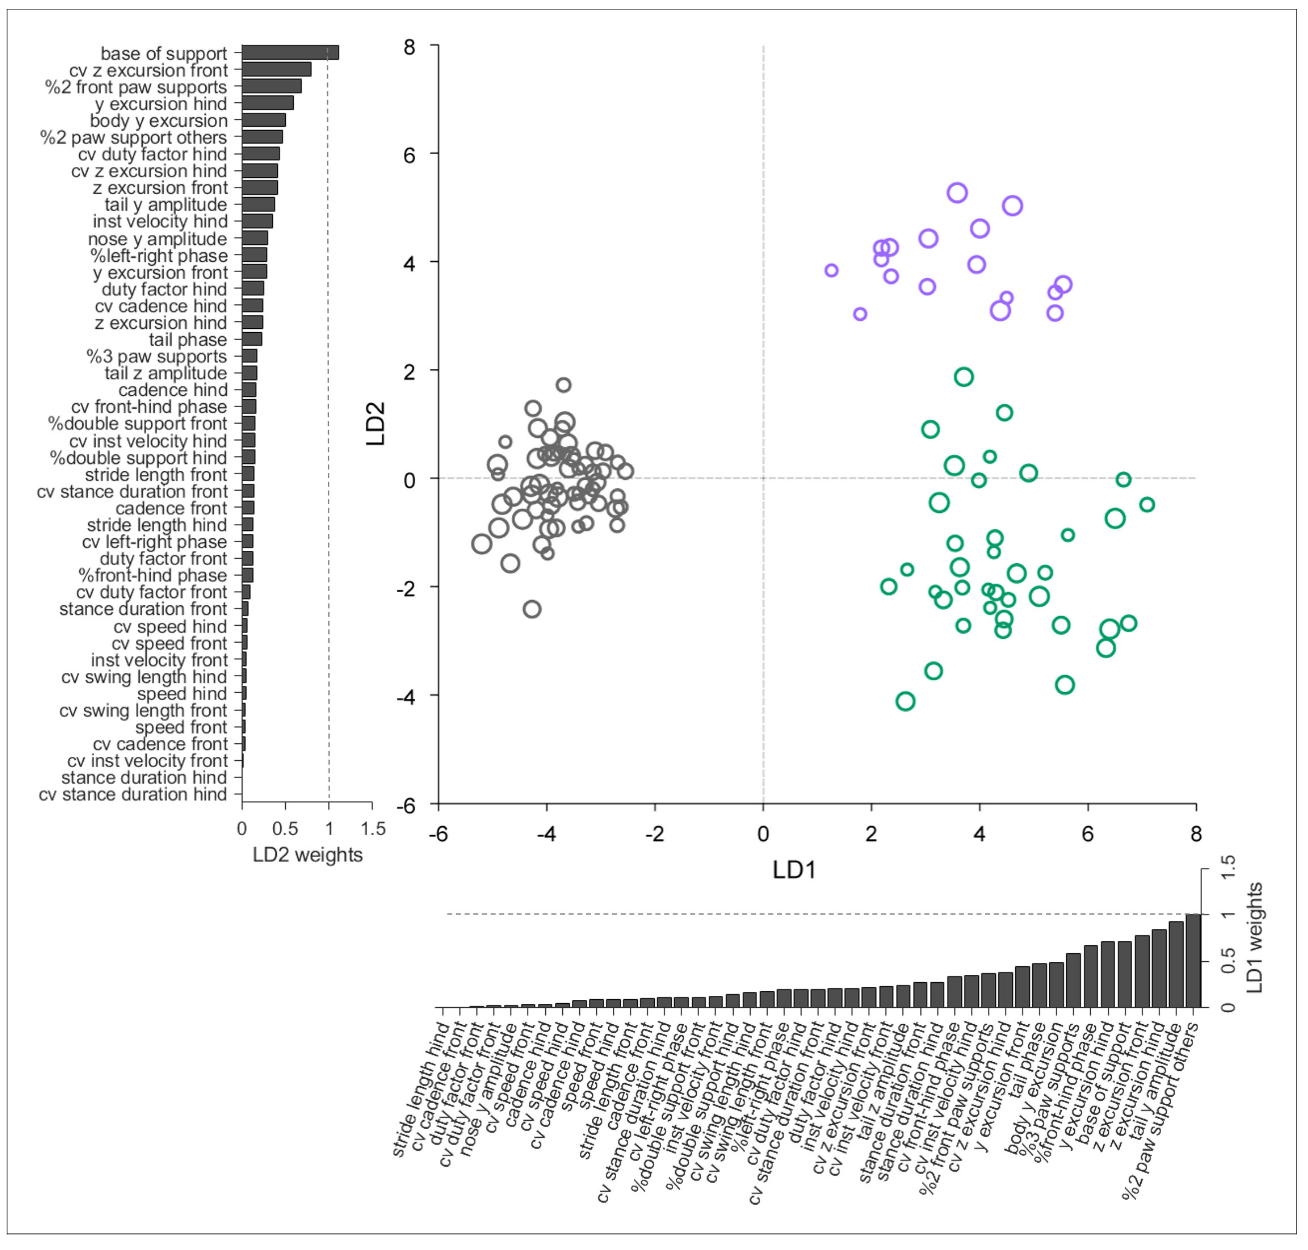
\includegraphics[width=1\linewidth]{Chapters//Figures//chapter2/LDA.png}
    \caption{Linear discriminant analysis of locomotor kinematics reveals two axes, which separate ataxic mutants from controls (LD1) and from each other (LD2). Each dot represents a single animal walking at a particular speed. Faster speeds are shown with larger marker sizes. Speeds ranged from 0.05 to 0.35 m/s and were binned with a bin width of 0.05 m/s. Size-matched controls are in grey (N = 11 for all speed bins; n = ~ 3288), reeler in green (N = 7 for 0.05–0.15 m/s; N = 6 for 0.25–0.35 m/s; n = ~ 2387), and pcd in purple (N = 3 for all speed bins except 0.25–0.30 m/s N = 2; n = ~ 3066). The bars along each axis are ranked by the contribution scores (LD coefficients) of each variable to that axis (larger bars indicate higher contributions). Features contributing strongly to LD1 (which accounts for 84\% of the total between-group variance) include interlimb and whole-body coordination, as well as off-axis paw trajectories. For LD2 (which accounts for 16\% of the between-group variance), they also include variability, front paw supports, and relative phasing of tail/nose movements.\\ Reproduced from Machado et al. 2020 \cite{machado_shared_2020}.}
    \label{fig:LDA}
\end{figure}

Locomouse was later used to analyze how 

\subsection{Animal models of cerebellar ataxia: PCD and Reeler mutants} % (fold)
\subsection{Behavior tracking in Locomouse}
\subsection{Quantification of locomotor parameters} % (fold)
\subsection{Linear discriminant analysis} % (fold)



% \section{Behavioral quantification}
% \section{Results}


\subsection{Low dimensional representation of kinematics}

\begin{figure}[h!]
    \centering
    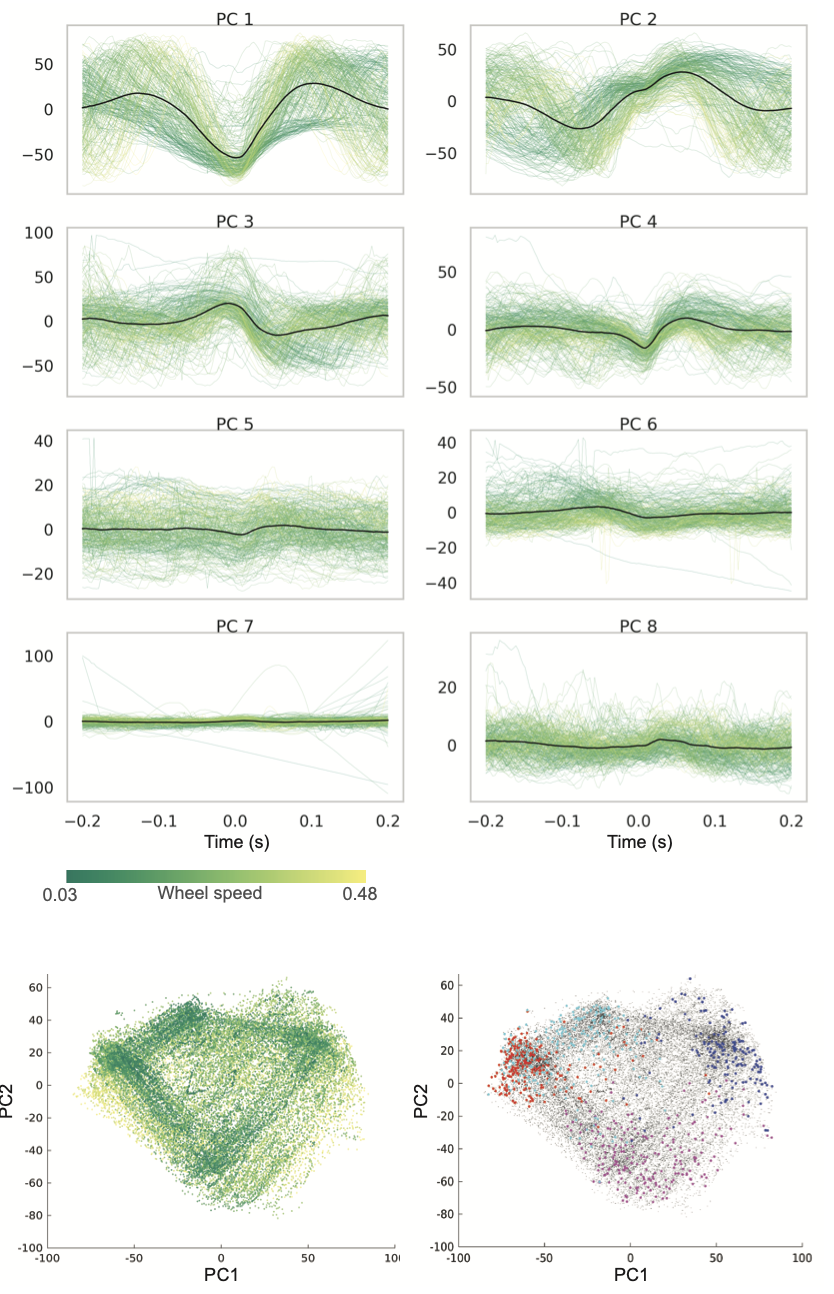
\includegraphics[width=1\linewidth]{Chapters//Figures//chapter2/behavioral_PCA.png}
    \caption{Principal component projections of instantaneous paw positions}
    \label{fig:behav-pca}
\end{figure}

\section{Discussion}


% \section{Locomotion lies on a cyclical manifold in low dimension}
% \subsection{Principal component analysis of instantaneous body positions} % (fold)
% \subsection{Low dimensional representations of locomotion} % (fold)
% \subsection{Encoding of locomotor phase and speed} % (fold)

% \section{Exploring locomotor cycle stereotipy}
